% VYSOKOŠKOLSKÁ KVALIFIKAČNÍ PRÁCE
% autor: 
% název: 
% kódování zdroje: UTF-8

\documentclass[a4paper,12pt]{article}

% test angličtiny \PassOptionsToPackage{main=english}{babel}

% globální nastavení pro text VŠKP UPa
\usepackage[
    % zakomentovat obojí biblatex= pro manuálně tvořený seznam literatury
	%biblatex=num,		% používat biblatex, číslované reference
	biblatex=harvard,	% harvardský styl citací v BibLaTeXu
	pdfa,				% použít \usepackage[a-1b]{pdfx} pro PDF/A
	writexmp,			% pro PDF/A: zapsat soubor XMP s metadaty dle \author, \title, \keywordsCZ
	%otf,				% fonty Open Type
]{vskpupa}				% globální nastavení pro text VŠKP UPa

%%%%%%%%%%%%%%%%%%%%%%%%%%%%%%%%%%%%%%%%%%%%%%%%%%%%%%%%%%%%
% ÚDAJE O PRÁCI, budou uvedeny v PDF /Info
%%%%%%%%%%%%%%%%%%%%%%%%%%%%%%%%%%%%%%%%%%%%%%%%%%%%%%%%%%%%

\author{Tymofii Voronkin}				% autor
\title{Rozšíření webového prohlížeče pro interaktivní náhledy souborů}			% název
%\thesisType{Diplomová práce}			% typ práce
\thesisType{Bakalářská práce}			% typ práce
\thesisYear{2026}						% rok odevzdání
\university{Univerzita Pardubice}		% univerzita
\faculty{% odkomentovat správný název fakulty
% Fakulta filozofická
% Dopravní fakulta Jana Pernera
% Fakulta ekonomicko-správní
% Fakulta chemicko-technologická
Fakulta elektrotechniky a informatiky
% Fakulta restaurování
% Fakulta zdravotnických studií
}

%%%%%%%%%%%%%%%%%%%%%%%%%%%%%%%%%%%%%%%%%%%%%%%%%%%%%%%%%%%%
% NASTAVENÍ BIBLIOGRAFIE
%%%%%%%%%%%%%%%%%%%%%%%%%%%%%%%%%%%%%%%%%%%%%%%%%%%%%%%%%%%%

\ifVSKPusesBibLaTeX
\ExecuteBibliographyOptions{
% nezle měnit zde: backend, style (bibstyle, citestyle)
	%%sorting=none,						% none → podle pořadí odkazů na zdroje
	%%sortlocale=cs_CZ,					% řazení dle abecedy v tomto jazyce
	%%bibencoding=auto,					% auto = (jako .tex), UTF8
	%autolang=other, 					% none|other – other = nastaví jazyk pro sazbu zdroje dle zdroje (podle langid)
	%maxnames=9, 						% maximální počet jmen
	%minnames=3, 						% je-li autorů více než maxnames, použije se jen minnames
	%maxcitenames=1,						% maximální počet jmen v citaci (harvardský styl)
	%mincitenames=1,
	%datezeros=false,					% nuly (pouze formáty short a terse)
	%date=short,
	%%date=comp, 						% iso = yyyy-mm-dd, comp: plné (dle jazyka)
	%%alldates=comp, 					% date, origdate, eventdate, urldate
	%%urldate=edtf,						% (BibLaTeX ≥ 3.10: iso) formát pro datum citace
	%dateabbrev=false,					% zkrácený formát (pouze formáty long a comp)
	%datecirca=true, 			    	% \datecircaprint před hrubým datem?
	%dateuncertain=true, 				% \(end)dateuncertainprint za nejistým datem?
	%% pokud je v souboru bib např.: date = 1790?, date = 1700~ %(cca)
	%shortnumeration=true,				% pro časopisy: true → svazek/ročník sázet tučně, číslo do závorky, false → slovně
	%thesisinfoinnotes=false,			% false → typ VŠKP práce, instituce a vedoucí PŘED dostupnost (odkaz), true → jako poznámku v citaci (na konec)
	%block=ragged,						% \raggedright pro bibliografii
	%giveninits=true,					% pouze iniciály jmen
	%uniquename=init,					% unikátní jméno počítá jen s iniciálami
	%abbreviate=true,					% zkratky
}

% změna textů pro českou verzi
\DefineBibliographyStrings{czech}{%
	%urlfrom = {dostupné z},
	urlfrom = {URL\addcolon},
	pages = {str\addabbrvspace},
}

% v seznamu místo obyčejného číslování (číslo s tečkou) použít hranaté závorky: 
\DeclareFieldFormat{labelnumberwidth}{\mkbibbrackets{#1}}

% první jméno FAMILY, Given a další jména Given FAMILY:
\DeclareNameAlias{author}{family-given/given-family}
\DeclareNameAlias{editor}{family-given/given-family}

%\DeclareNameAlias{translator}{given-family}
%\DeclareNameAlias{byeditor}{given-family}
%\DeclareNameAlias{bytranslator}{given-family}

% BibLaTeX: změna oddělovače jmen: výchozí je středník (;), změněno ve stylu na:
%	čárka (harvardský styl) v odkazech (cicacích)
%	v seznamu literatury pak středník + spojka „a“

% globálně (zejména odkazy):
%\renewcommand\multinamedelim{\addsemicolon\space}			% středník
%\renewcommand\multinamedelim{\addcomma\space}				% čárka

% pouze v seznamu literatury:
\AtBeginBibliography{%
	% změna oddělovače jmen: výchozí je středník (;):
	%\renewcommand\multinamedelim{\addsemicolon\space}		% středník
	%\renewcommand\multinamedelim{\addcomma\space}%			% čárka
	\renewcommand\multinamedelim{\addnbspace--\addspace}%	% pomlčka
	\renewcommand\finalnamedelim{\addspace\bibstring{and}\addnbspace}%	% mezi předposlední a poslední jméno
}

% odkazy na více zdrojů: penalta za zlom mezi jednotlivými čísly v závorce
%\setcounter{multicitedelimpenalty}{1000}
%\setcounter{multicitefinaldelimpenalty}{10000}

% zákaz dělení slov v seznamu literatury
%\appto\bibsetup{\hyphenpenalty=10000 }

% zmenšit font pro seznam zdrojů
%\renewcommand*{\bibfont}{\footnotesize}

\addbibresource{references.bib}			% seznam zdrojů

\fi	% používání BibLaTeXu

% DODATEČNÁ NASTAVENÍ

% zalamování URL:
% \resetURLchars						% vypne všechny zalamovací znaky (z url.sty)
% \setURLbreaks*	{/{2}}	{&}			% přednostně za / (od 3. výskytu) a před &
% \setURLbreaks	{:{1}}	{?+#}		% za : (od 2.výskytu) a před ?, + a #

\renewcommand\arraystretch{1.1}		% rozestup linek tabulek

\definecolor{red}{cmyk}{0,1,1,.1}	% redefinice červené barvy (tmavěji)
\definecolor{green}{cmyk}{1,0,1,.1}	% redefinice zelené barvy (tmavěji)

% často je vhodné výčty nezarovnávat na pravý okraj
%\setlist*[itemize,enumerate,description]{
%	%before=\raggedright,				% nezarovnávat pravý okraj ve výčtech
%}

%\setcounter{secnumdepth}{3} 			% číslovat titulky pouze do této úrovně
%\setcounter{tocdepth}{3}				% obsah generovat až do této úrovně

 
%%%%%%%%%%%%%%%%%%%%%%%%%%%%%%%%%%%%%%%%%%%%%%%%%%%%%%%%%%%%
% NASTAVENÍ HYPERTEXTOVÝCH ODKAZŮ V PDF
%%%%%%%%%%%%%%%%%%%%%%%%%%%%%%%%%%%%%%%%%%%%%%%%%%%%%%%%%%%%

% a) výchozí nastavení: rámečky kolem textu, které se netisknou

% b) bez rámečků, odkomentovat:
%\hypersetup{hidelinks}

% c) bez rámečků, barevně, odkomentovat:
\hypersetup{
	colorlinks=true, 					% zapnout barvy, vypnout rámečky
%	% nastavit barvy samostatně:
%	linkcolor=red,						% interní odkazy (křížové reference)
%	anchorcolor=black,					% text kotvy
%	citecolor=green,					% text odkazu na citaci
%	filecolor=cyan,						% URL pro lokální soubory
%	urlcolor=magenta,					% URL
%	% nebo nastavit všechny barvy stejně:
%	%allcolors=blue, 					% všechny odkazy (netýká se rámečků)
}

% další vlastní nastavení uživatele

%%%%%%%%%%%%%%%%%%%%%%%%%%%%%%%%%%%%%%%%%%%%%%%%%%%%%%%%%%%%
% ÚDAJE O PRÁCI
%%%%%%%%%%%%%%%%%%%%%%%%%%%%%%%%%%%%%%%%%%%%%%%%%%%%%%%%%%%%

% cesty k obrázkům naskenovaného zadání
% jména souborů budou tvořena jako \prefixZadani #\suffixZadani
% místo # se doplní pořadové číslo obrázku (začíná se jedničkou)
\def\prefixZadani{img/zadani}			% cesta a začátek jména, bude doplněno číslo strany
\def\suffixZadani{.jpg}					% doplní se ke každému jménu souboru zadání

\def\datumOdevzdaniPrace{6.\,5.\,2026}	% datum pod prohlášením

% nutné pouze pro vzor pro vkládání výplňkových textů
\usepackage{lipsum}						% \lipsum[číslo] vloží jeden odstavec Lorem ipsum…
\usepackage{graphicx}
\usepackage{pdfpages}					% vkládání stránek z externího PDF
\usepackage{subcaption}                 % Pro vedle sebe umístěné obrázky
% \usepackage{listings}     % už načteno stylem VŠKP (vskpupa.sty, czechtypo.sty)
\lstset{
  language=JavaScript,
  basicstyle=\ttfamily\small,
  keywordstyle=\color{blue}\bfseries,
  stringstyle=\color{red},
  commentstyle=\color{green!50!black},
  showstringspaces=false,
  frame=single,
  numbers=left,
  numberstyle=\tiny\color{gray},
  breaklines=true,
  captionpos=b,
  escapeinside={\%(*}{*)},
  %texcl=true,
}

% PROHLÁŠENÍ O VYUŽITÍ UMĚLÉ INTELIGENCE (Úroveň 2)
\long\def\textProhlaseniAI{%
	Při přípravě této práce byly využity nástroje umělé inteligence (zejména velké jazykové modely) v~souladu s~pravidly Univerzity Pardubice (Úroveň 2). Konkrétně byly použity modely \textit{Google Gemini 3.1 Pro} a~\textit{Anthropic Claude Sonnet 4.6}. Nástroje AI byly použity výhradně k~dílčím úkonům:
	\begin{itemize}
		\item Asistence při návrhu softwarové architektury,
		\item Generování, úprava a~kontrola částí zdrojového kódu (rozšíření prohlížeče),
		\item Gramatická korektura a~stylistická úprava textu.
	\end{itemize}
	Za konečný obsah a~výsledky práce nesu plnou zodpovědnost.
}

% PODĚKOVÁNÍ
\long\def\textPodekovani{%
	Rád bych poděkoval vedoucímu své bakalářské práce, Mgr. Tomáši Hudcovi, za odborné vedení, cenné rady a~čas, který mi věnoval při konzultacích.

	Zvláštní poděkování patří mým přátelům, kteří byli vždy po mém boku~-- podporovali mě, pomáhali mi v~těžkých chvílích a~nikdy nenechali chvíle smutku trvat příliš dlouho. Jejich přítomnost pro mě znamená víc, než dokáži slovy vyjádřit.

	Děkuji svému otci za vše, co do mě vložil~-- zejména za lásku k~počítačům a~informačním technologiím, kterou ve mně probouzel od nejútlejšího věku. Díky němu jsem našel cestu, po které dnes kráčím.

	Děkuji své mladší sestře, která mi byla oporou a~radostí zároveň~-- a~která nedovolila, aby mé vnitřní dítě úplně zaniklo.

	Zvláštní, hluboký dík patří mé mamince~-- člověku, který ve mě věřil za všech okolností, od dětství mě učil nevzdávat se a~důvěřovat vlastní cestě. Je mi nesmírně líto, že se nedočká mé promoce ani dalšího dospívání po mém boku. \textit{Světlé památce.}
}
% ANOTACE
\long\def\anotace{%
	Tato bakalářská práce se zabývá návrhem a~implementací rozšíření pro webové prohlížeče (Google Chrome a~Mozilla Firefox), které zvyšuje efektivitu prohlížení webových stránek. Rozšíření umožňuje okamžité zobrazení náhledů obrázků a~dokumentů PDF pouhým najetím kurzoru myši na příslušný odkaz, čímž eliminuje nutnost stahování souborů a~otevírání nových oken. Teoretická část popisuje architekturu rozšíření (Manifest~V3), asynchronní programování v~jazyce JavaScript a~práci s~knihovnou PDF.js. Praktická část detailně analyzuje implementaci logiky rozšíření, tvorbu uživatelského rozhraní s~podporou filtrování domén pomocí regulárních výrazů a~následné testování na reálných webových stránkách.
}
% KLÍČOVÁ SLOVA
\keywordsCZ{rozšíření prohlížeče, JavaScript, interaktivní náhledy, PDF.js, asynchronní programování, Manifest V3}

% ENGLISH TITLE
\def\titleEN{Web Browser Extension for Interactive File Previews}
% ENGLISH ANNOTATION
\long\def\annotation{%
	This bachelor thesis deals with the design and implementation of a~web browser extension (for Google Chrome and Mozilla Firefox) that increases the efficiency of web browsing. The extension allows for instant previews of images and PDF documents simply by hovering the mouse cursor over the relevant link, eliminating the need to download files or open new windows. The theoretical part describes the architecture of extensions (Manifest~V3), asynchronous programming in JavaScript, and working with the PDF.js library. The practical part analyzes in detail the implementation of the extension's logic, the creation of a user interface with support for domain filtering using regular expressions, and subsequent testing on real websites.
}
% ENGLISH KEYWORDS
\keywordsEN{browser extension, JavaScript, interactive previews, PDF.js, asynchronous programming, Manifest V3}


%%%%%%%%%%%%%%%%%%%%%%%%%%%%%%%%%%%%%%%%%%%%%%%%%%%%%%%%%%%%
% ZAČÁTEK DOKUMENTU
%%%%%%%%%%%%%%%%%%%%%%%%%%%%%%%%%%%%%%%%%%%%%%%%%%%%%%%%%%%%

\begin{document}

%%%%%%%%%%%%%%%%%%%%%%%%%%%%%%%%%%%%%%%%%%%%%%%%%%%%%%%%%%%%
% ÚVODNÍ STRANY
%%%%%%%%%%%%%%%%%%%%%%%%%%%%%%%%%%%%%%%%%%%%%%%%%%%%%%%%%%%%

\titulniStrana							% titul

%%%%%%%%%%%%%%%%%%%%%%%%%%%%%%%%%%%%%%%%%%%%%%%%%%%%%%%%%%%%
% ZADÁNÍ

\pagestyle{plain}

% zadání vloženo přímo z PDF pomocí pdfpages (zachovává vektorovou kvalitu):
\clearpage
    
\phantomsection\label{assignment}
\pdfbookmark[1]{Zadání}{assignment}
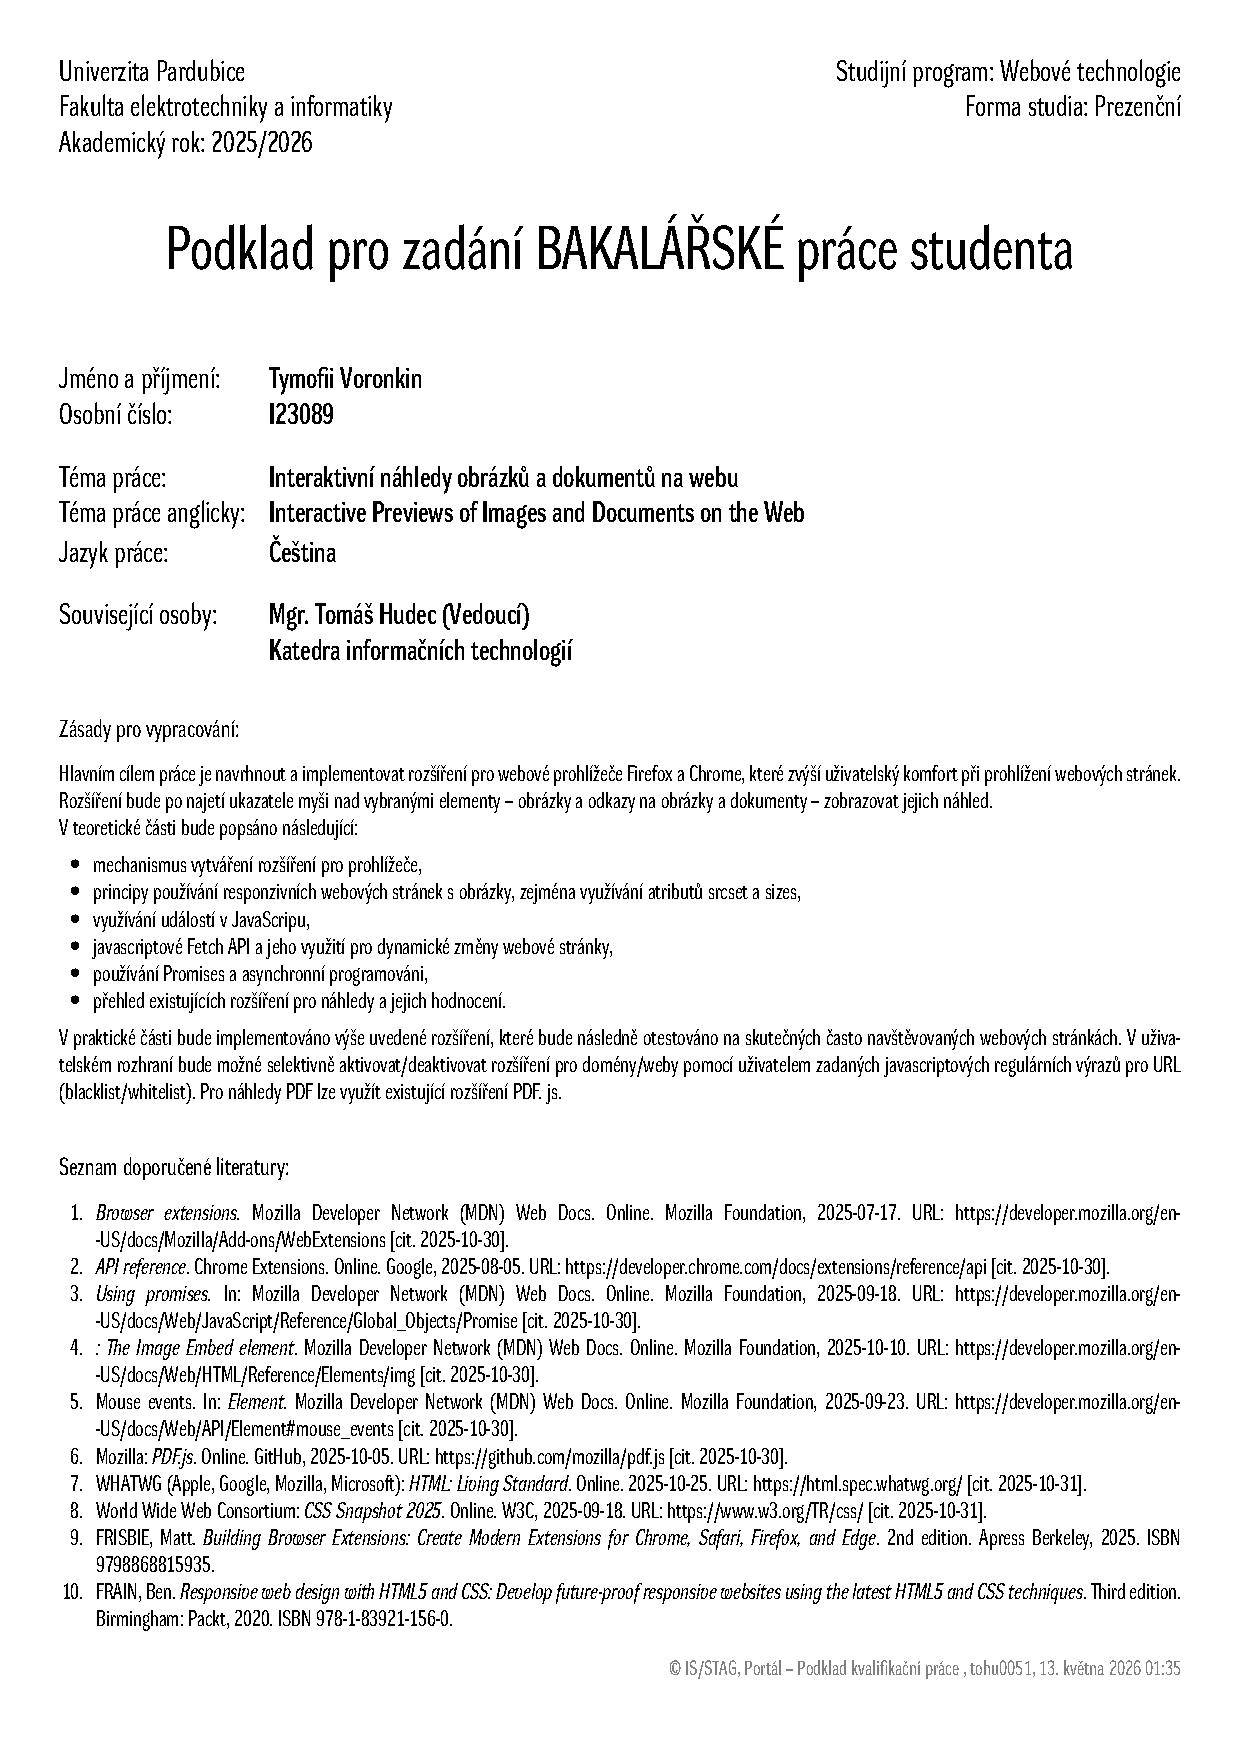
\includepdf[
	pages=-,
	pagecommand={},
	width=\textwidth,
]
{img/Zadani-BP-Voronkin-names-flatten.pdf}
%{img/Zadani-BP-Voronkin-signed.pdf}

% alternativy:
	%\generujZadani[2]					% vložení pomocí obrázků (img/zadani1.jpg, …)
	%\addtocounter{page}{2}				% pouze započítat strany bez vložení
	%\vakatZadani[2]					% prázdné stránky (vakáty)

\generujProhlaseni						% prohlášení, [z] pro ženský rod
% \podekovaniDolu						% odkomentovat, pokud má být poděkování vespod stránky

% VLOŽENÍ PROHLÁŠENÍ O VYUŽITÍ AI (vlastní úprava pod standardní prohlášení)
\clearpage
\vspace*{\fill}
\noindent\textbf{Prohlášení o~využití umělé inteligence}\\[1em]
\textProhlaseniAI
\vspace{2cm}

\generujPodekovani						% poděkování
\generujAnotaci							% anotace
% \clearpage							% odkomentovat, má-li být anglická anotace na následující straně
\generujAnnotation						% anotace anglicky
\generujObsah							% obsah
\generujSeznamObrazku					% seznam obrázků
% seznam tabulek záměrně vynechán – práce neobsahuje žádné tabulky

%%%%%%%%%%%%%%%%%%%%%%%%%%%%%%%%%%%%%%%%%%%%%%%%%%%%%%%%%%%%
% SEZNAM ZKRATEK

\seznamZkratek							% titulek a řádek do obsahu

\begin{description}[
	font=\mdseries, 
	leftmargin=4.3em,
	labelwidth=!,
	before=\raggedright,
]
\item[AJAX]		Asynchronous JavaScript and XML – asynchronní JavaScript a~XML
\item[API]		Application Programming Interface – rozhraní pro programování aplikací
\item[CORS]		Cross-Origin Resource Sharing – mechanismus sdílení zdrojů napříč doménami
\item[CSS]		Cascading Style Sheets – kaskádové styly
\item[CSP]		Content Security Policy – bezpečnostní politika obsahu
\item[DOM]		Document Object Model – objektový model dokumentu
\item[FEI]		Fakulta elektrotechniky a~informatiky
\item[HTML]		HyperText Markup Language – značkovací jazyk pro webové stránky
\item[HTTP]		HyperText Transfer Protocol – protokol pro přenos hypertextu
\item[IS STAG]	Informační systém Studijní agenda
\item[JS]		JavaScript – skriptovací jazyk pro webové aplikace
\item[JSON]		JavaScript Object Notation – formát pro výměnu dat
\item[MIME]		Multipurpose Internet Mail Extensions – typ internetového média
\item[MV3]		Manifest Version 3 – specifikace Manifest V3
\item[PDF]		Portable Document Format – přenosný formát dokumentů
\item[SVG]		Scalable Vector Graphics – škálovatelná vektorová grafika
\item[UI]		User Interface – uživatelské rozhraní
\item[UPCE]		Univerzita Pardubice
\item[URL]		Uniform Resource Locator – jednotný lokátor zdrojů
\item[UX]		User Experience – uživatelský prožitek
\item[XMP]		Extensible Metadata Platform – rozšiřitelná platforma pro metadata
\end{description}


%%%%%%%%%%%%%%%%%%%%%%%%%%%%%%%%%%%%%%%%%%%%%%%%%%%%%%%%%%%%
% ÚVOD
%%%%%%%%%%%%%%%%%%%%%%%%%%%%%%%%%%%%%%%%%%%%%%%%%%%%%%%%%%%%

\clearpage\pagestyle{plain}				% zapne číslování stránek (sazba zápatí)

%%%%%%%%%%%%%%%%%%%%%%%%%%%%%%%%%%%%%%%%%%%%%%%%%%%%%%%%%%%%
%%%%%%%%%%%%%%%%%%%%%%%%%%%%%%%%%%%%%%%%%%%%%%%%%%%%%%%%%%%%
\section*{Úvod}
\label{sec:uvod}
 
V~současné digitální éře představuje webový prohlížeč nejdůležitější bránu k~informacím. Denně uživatelé projdou desítky až stovky webových stránek, přičemž se neustále setkávají s~obrovským množstvím hypertextových odkazů, obrázků a~dokumentů. 

Tradiční způsob interakce s~tímto obsahem obvykle vyžaduje aktivní kliknutí na odkaz a~načtení nové stránky nebo stažení souboru na lokální disk před jeho samotným zobrazením. Tento proces je nejen časově náročný, ale také narušuje plynulost práce (tzv.~\textit{workflow}) a~zbytečně plní úložiště uživatele staženými soubory, které byly potřeba jen pro rychlé nahlédnutí.

S~narůstajícím tempem konzumace obsahu roste i~poptávka po efektivnějších způsobech procházení webu. Jedním z~možných řešení tohoto problému jsou rozšíření pro webové prohlížeče (tzv.~\textit{browser extensions}), která dokážou modifikovat chování webových stránek a~přidávat nové funkce přímo do uživatelského rozhraní prohlížeče.

Cílem této bakalářské práce je navrhnout, implementovat a~otestovat právě takové softwarové řešení~-- moderní rozšíření pro webové prohlížeče (zaměřené na platformy Google Chrome a~Mozilla Firefox), které uživatelům umožní okamžité zobrazení náhledů obrázků a~dokumentů (zejména formátu PDF). 

Rozšíření funguje na principu aktivace při pouhém najetí kurzoru myši (událost \textit{hover}) nad vybraný webový element, čímž eliminuje nutnost klikání či otevírání nových panelů. 

Tato práce je rozdělena na dvě hlavní části. V~teoretické části (viz kapitola~\ref{sec:teorie}) jsou detailně rozebrány mechanismy a~principy nezbytné pro vývoj takového rozšíření. Čtenář je seznámen s~architekturou rozšíření prohlížečů postavenou na specifikaci Manifest~V3, technikami responzivního webového designu (s~důrazem na práci s~obrázky pomocí atributů \texttt{srcset} a~\texttt{sizes}) a~obsluhou asynchronních událostí v~jazyce JavaScript. 

Důležitá pozornost je věnována také moderním přístupům získávání dat přes rozhraní Fetch API a~využití \textit{Promises}. Na závěr teoretické části je provedena analýza a~zhodnocení existujících konkurenčních řešení, což slouží jako východisko pro vlastní implementaci.

Praktická část (viz kapitola~\ref{sec:praxe}) pak popisuje konkrétní realizaci navrženého rozšíření. Zabývá se softwarovou architekturou projektu, implementací logiky detekce odkazů a~tvorbou uživatelského rozhraní, které mimo jiné nabízí možnost pokročilé konfigurace domén pomocí regulárních výrazů (systém \textit{Blocklist/Allowlist}). 

Významná podkapitola je věnována integraci knihovny PDF.js pro bezpečné a~plynulé renderování dokumentů PDF přímo v~prohlížeči. Práce je zakončena kapitolou shrnující testování rozšíření v~reálných podmínkách na frekventovaných webových stránkách a~zhodnocením dosažených výsledků.

%%%%%%%%%%%%%%%%%%%%%%%%%%%%%%%%%%%%%%%%%%%%%%%%%%%%%%%%%%%%
% TEORETICKÁ ČÁST
%%%%%%%%%%%%%%%%%%%%%%%%%%%%%%%%%%%%%%%%%%%%%%%%%%%%%%%%%%%%

\section{Teoretická část}
\label{sec:teorie}

V~této části je teoreticky popsán mechanismus fungování webových rozšíření a~použité technologie.

\subsection{Mechanismus vytváření rozšíření pro prohlížeče}
\label{subsec:teorie_rozsireni}

Rozšíření prohlížeče (anglicky \textit{browser extension}) je malý softwarový modul, který přizpůsobuje zážitek z~prohlížení webu. Rozšíření umožňují uživatelům přizpůsobit funkcionalitu a~chování prohlížeče individuálním potřebám nebo preferencím~\autocite{mdn_extensions}. Moderní rozšíření jsou budována pomocí standardních webových technologií, tedy jazyka HTML, kaskádových stylů (CSS) a~jazyka JavaScript~\autocite{flanagan2020}. Většina současných prohlížečů, včetně Google Chrome, Mozilla Firefox, Microsoft Edge a~Safari, podporuje unifikovaný standard WebExtensions API, díky kterému lze napsat kód jednou a~s~minimálními úpravami jej zkompilovat pro různé platformy~\autocite{frisbie2025}.

Historicky byla většina rozšíření postavena na architektuře Manifest~V2. Vzhledem k~rostoucím obavám o~soukromí uživatelů a~bezpečnost však společnost Google představila novou specifikaci Manifest~V3, která se stala novým průmyslovým standardem. Hlavním rozdílem mezi~V2 a~V3 je přesun od tzv.~\textit{Background Pages} (stránek na pozadí, které běžely neustále a~zabíraly operační paměť) k~\textit{Service Workerům}, které jsou probouzeny pouze na základě specifických událostí. Tím se výrazně snižuje paměťová náročnost rozšíření. Další klíčovou změnou je přísnější bezpečnostní model, který zakazuje spouštění vzdáleně hostovaného kódu (remote code execution) a~omezuje pravidla pro blokování síťových požadavků přes \texttt{webRequest} API, což nutí vývojáře využívat nové deklarativní API~\autocite{chrome_api}.

Klíčovým stavebním kamenem každého rozšíření je konfigurační soubor s~názvem \texttt{manifest.json}. Tento soubor definuje základní metadata aplikace (název, verzi, popis), požadovaná oprávnění (např.~přístup k~aktivní záložce přes \texttt{activeTab} nebo oprávnění k~ukládání dat přes \texttt{storage}) a~deklaruje komponenty, ze kterých se rozšíření skládá.

Architektura běžného rozšíření se skládá z~několika oddělených, avšak vzájemně komunikujících komponent~\autocite{frisbie2025}:
\begin{itemize}
    \item \textbf{Content Scripts (Skripty obsahu):} Tyto javascriptové soubory jsou injektovány přímo do kontextu webových stránek, které uživatel navštíví. Mohou číst a~upravovat Document Object Model (DOM) dané stránky, což je nezbytné pro detekci prvků (např.~odkazů nebo obrázků) a~modifikaci uživatelského rozhraní přímo na prohlíženém webu. Sdílejí DOM s~originální stránkou, ale jejich spouštěcí prostředí a~proměnné jsou izolované.
    \item \textbf{Background Scripts (Skripty na pozadí):} V~rámci Manifestu V3 jsou realizovány prostřednictvím tzv.~\textit{Service Workerů}. Běží nezávisle na životním cyklu webové stránky, reagují na systémové události prohlížeče (jako je např.~kliknutí na ikonu rozšíření, instalace aktualizace) a~mohou udržovat dlouhodobý stav. Tyto skripty nemají přímý přístup k~DOMu žádné stránky, a~proto musí s~Content Skripty komunikovat přes mechanismus zpráv (Message Passing)~\autocite{chrome_api}.
    \item \textbf{Uživatelské rozhraní (Popup a~Options):} Většina rozšíření disponuje viditelným grafickým rozhraním. \textit{Popup} se zobrazí při kliknutí na ikonu rozšíření v~liště prohlížeče a~slouží k~rychlým interakcím. Stránka \textit{Options} (Možnosti) poskytuje komplexnější prostředí pro konfiguraci rozšíření, přičemž uživatelská nastavení se obvykle ukládají pomocí \texttt{chrome.storage} API, odkud je následně mohou asynchronně načítat ostatní komponenty.
\end{itemize}

Omezení přístupových práv (\textit{Permissions}) představuje jeden z~nejdůležitějších bezpečnostních konceptů při vývoji rozšíření. Na rozdíl od běžných webových stránek mohou rozšíření po udělení souhlasu přistupovat k~citlivým funkcím operačního systému prohlížeče, např.~obcházet pravidla CORS (Cross-Origin Resource Sharing) pro asynchronní požadavky na vzdálené servery~\autocite{mdn_extensions}. Toto je klíčové pro aplikace stahující dodatečný obsah na pozadí, aniž by došlo k~blokování požadavku ze strany bezpečnostních mechanismů samotné prohlížené stránky.

\subsection{Principy responzivních webových stránek s~obrázky}
\label{subsec:teorie_responzivni}

Při vývoji rozšíření pro zobrazování náhledů obrázků je klíčové porozumět moderním technikám vkládání grafiky do HTML dokumentu. V~minulosti vývojáři spoléhali výhradně na atribut \texttt{src} u~značky \texttt{<img>}. S~nástupem mobilních zařízení s~displeji o~vysoké hustotě pixelů (např. Retina displeje) však vznikla potřeba responzivního načítání obrázků~\autocite{frain2020}. 

Moderní specifikace HTML~\autocite{whatwg_html} zavedla dva klíčové atributy pro element \texttt{<img>}, a~to \texttt{srcset} a~\texttt{sizes}, případně samostatný element \texttt{<picture>}. Atribut \texttt{srcset} obsahuje čárkou oddělený seznam adres obrázků spolu s~jejich šířkou (např.~\texttt{image-800w.jpg 800w}). Atribut \texttt{sizes} pak definuje, jaký prostor bude obrázek na obrazovce zabírat v~závislosti na tzv.~\textit{media queries} (např.~\texttt{(max-width:~600px) 100vw, 50vw}). Prohlížeč následně sám asynchronně vyhodnotí velikost okna, hustotu pixelů displeje a~z~atributu \texttt{srcset} stáhne nejvhodnější obrázek~\autocite{mdn_img}. 

Z~hlediska vývoje rozšíření, které má po najetí myší zobrazit zvětšený náhled obrázku, to znamená, že se nelze spolehnout pouze na hodnotu atributu \texttt{src}, protože ta může obsahovat pouze \textit{fallback} (záložní obrázek) v~nízkém rozlišení. Namísto toho musí rozšiřující skript analyzovat atribut \texttt{srcset} nebo nadřazené značky \texttt{<source>} a~extrahovat URL adresu obrázku s~nejvyšším možným rozlišením.

\subsection{Využívání událostí v~JavaScriptu}
\label{subsec:teorie_udalosti}

Aby rozšíření dokázalo reagovat na činnost uživatele~-- konkrétně na pohyb myši nad vybranými elementy~-- je nutné využít systém událostí (tzv.~\textit{Event Handling}) v~rámci modelu~DOM. JavaScript komunikuje s~dokumentem~HTML asynchronně prostřednictvím posluchačů událostí (\texttt{EventListeners})~\autocite{flanagan2020}. 

Pro účely náhledového rozšíření jsou klíčové události související s~pohybem kurzoru~\autocite{mdn_mouse}:
\begin{itemize}
    \item \texttt{mouseover} a~\texttt{mouseout}: Tyto události jsou vyvolány, když kurzor vstoupí do oblasti elementu, respektive ji opustí. Jejich specifikem je, že tzv.~\textit{probublávají} (Event Bubbling) směrem nahoru strukturou DOMu k~nadřazeným elementům. Toho lze využít pro efektivní zachytávání událostí na celém dokumentu (tzv.~\textit{Event Delegation}) namísto vázání samostatného posluchače na každý jednotlivý obrázek či odkaz na stránce.
    \item \texttt{mouseenter} a~\texttt{mouseleave}: Podobné jako předchozí, avšak s~tím rozdílem, že neprobublávají. K~vyvolání dojde pouze tehdy, když kurzor myši fyzicky překročí hranici elementu, na kterém je posluchač navázán~\autocite{mdn_mouse}.
    \item \texttt{mousemove}: Vyvolává se opakovaně po celou dobu, kdy se kurzor pohybuje uvnitř elementu. V~kontextu rozšíření se využívá k~průběžnému přepočítávání pozice (souřadnic $x$,~$y$) náhledového okna tak, aby plynule následovalo pohyb uživatelovy myši.
\end{itemize}

Vzhledem k~četnosti spouštění události \texttt{mousemove} je při implementaci nezbytné dbát na výkon a~využívat optimalizační techniky. Pokud by se při každém pohnutí myši nad prvkem asynchronně spouštěly složité výpočty nebo překreslování DOMu, mohlo by docházet k~zamrzání uživatelského rozhraní prohlížeče~\autocite{flanagan2020}. 

Nejčastěji se využívají návrhové vzory \textit{debounce} a~\textit{throttle}. Vzor \textit{debounce} zajišťuje, že se určitá funkce spustí až po uplynutí definované doby nečinnosti od posledního vyvolání události. To je ideální pro detekci záměrného najetí myší (tzv.~\textit{intent to hover}), nikoliv pouhého přejetí přes odkaz během posouvání stránky. Příklad takové implementace, kde je k~zobrazení náhledu využit časovač (timeout), ukazuje výpis~\ref{lst:debounce}.

\begin{lstlisting}[caption={Příklad jednoduché implementace funkce debounce pro odložení náhledu}, label={lst:debounce}]
function debounce(func, wait) {
    let timeout;
    return function(...args) {
        clearTimeout(timeout);
        timeout = setTimeout(() => func.apply(this, args), wait);
    };
}

// Použití pro zpožděné zobrazení náhledu po 500 ms
const linkElement = document.querySelector('a');
linkElement.addEventListener('mouseover', debounce(showPreview, 500));
\end{lstlisting}

\subsection{Javascriptové Fetch API}
\label{subsec:teorie_fetch}

Pro načtení obsahu cílového odkazu (např.~stažení PDF souboru) před jeho zobrazením v~náhledovém okně slouží asynchronní HTTP požadavky. V~minulosti byl za tímto účelem využíván objekt \texttt{XMLHttpRequest} (AJAX). Moderní vývoj však zcela přechází na rozhraní \textbf{Fetch API}, které poskytuje robustnější, flexibilnější a~logičtější způsob pro získávání síťových zdrojů~\autocite{flanagan2020}.

Globální metoda \texttt{fetch()} iniciuje proces stahování zdroje ze sítě a~na rozdíl od starších řešení vrací rovnou objekt typu \texttt{Promise} (slib), čímž elegantně řeší problémy spojené s~vnořováním asynchronních \textit{callback} funkcí. Použití Fetch API v~kombinaci s~\textit{Service Workery} rozšíření umožňuje elegantně stahovat bloky dat (např.~formou datových proudů~-- \textit{Streams}) i~z~domén, které by za normálních okolností blokovala politika stejného původu (Same-Origin Policy), a~tato data následně dynamicky injectovat do prohlížené webové stránky formou HTML či Canvas elementů.

\subsection{Používání Promises a~asynchronní programování}
\label{subsec:teorie_promises}

Běhové prostředí jazyka JavaScript je ve své podstatě jednovláknové (\textit{single-threaded}). Jakákoliv zdlouhavá operace (např.~stahování velkého dokumentu PDF) by v~synchronním režimu zablokovala hlavní vlákno a~způsobila zamrznutí celého uživatelského rozhraní prohlížeče. K~řešení tohoto problému slouží asynchronní programování~\autocite{flanagan2020}.

Základním kamenem moderní asynchronní logiky v~JavaScriptu je objekt \texttt{Promise} (česky příslib nebo slib). \texttt{Promise} reprezentuje hodnotu, která v~daném okamžiku ještě nemusí existovat, ale bude dostupná někdy v~budoucnosti~\autocite{mdn_promises}. Tento objekt se může nacházet ve třech stavech:
\begin{itemize}
    \item \textbf{pending (čekající):} Výchozí stav, asynchronní operace ještě nebyla dokončena.
    \item \textbf{fulfilled (splněný):} Operace byla úspěšně dokončena a~\texttt{Promise} obsahuje výslednou hodnotu.
    \item \textbf{rejected (zamítnutý):} Operace selhala (např.~chyba sítě, soubor nenalezen) a~\texttt{Promise} obsahuje důvod selhání (objekt chyby).
\end{itemize}

I~když API samotných \textit{Promises} (metody \texttt{.then()} a~\texttt{.catch()}) výrazně zlepšilo čitelnost kódu oproti starším metodám, novější specifikace ECMAScript představily syntaktický cukr v~podobě klíčových slov \texttt{async} a~\texttt{await}. Tato syntaxe umožňuje psát asynchronní kód tak, aby vypadal a~choval se jako klasický kód synchronní, což zásadně snižuje složitost logiky při vývoji komplexních rozšíření.

\subsection{Přehled existujících rozšíření pro náhledy a~jejich hodnocení}
\label{subsec:teorie_existujici}

Koncept interaktivních náhledů pomocí najetí myší (hover) není v~prostředí webových prohlížečů novinkou. Existuje několik zaběhnutých řešení, mezi nejznámější patří rozšíření \textit{Hover Zoom+} a~\textit{Imagus} (resp. jeho komunitní nástupce \textit{Imagus Reborn}). Tato řešení však trpí určitými nedostatky, které odůvodňují vývoj vlastního, moderního nástroje.

\subsubsection*{Rozšíření Hover Zoom+}
Rozšíření \textbf{Hover Zoom+} (viz obrázek~\ref{fig:hoverzoom}) je jedním z~historicky nejznámějších nástrojů v~této kategorii. Původní verze (Hover Zoom) měla v~minulosti vážné bezpečnostní problémy spojené se sledováním uživatelů a~vkládáním škodlivého kódu (spyware), což vedlo k~narušení důvěry komunity a~jejímu odstranění z~obchodů s~doplňky.

Současná verze se sice pyšní otevřeným zdrojovým kódem (open-source), avšak z~uživatelského hlediska trpí zastaralým designem a~nepřehledným rozhraním s~obrovským množstvím komplikovaných nastavení, ve kterých se běžný uživatel snadno ztratí. Navíc podpora dokumentů je velmi omezená a~zcela chybí vestavěná integrace pro náhledy souborů~PDF bez nutnosti instalace dalších externích modulů.

\begin{figure}[htbp]
    \centering
    \begin{subfigure}[b]{\textwidth}
        \centering
        \includegraphics[width=\textwidth]{img/competitors_Hover-Zoom_Chrome-Web-store.png}
        \caption{Chrome Web Store}
    \end{subfigure}
    
    \vspace{1.5em}
    \begin{subfigure}[b]{0.45\textwidth}
        \centering
        \includegraphics[width=\textwidth]{img/competitors_Hover-Zoom_Popup.png}
        \caption{Vyskakovací okno}
    \end{subfigure}
    \hfill
    \begin{subfigure}[b]{0.45\textwidth}
        \centering
        \includegraphics[width=\textwidth]{img/competitors_Hover-Zoom_Options.png}
        \caption{Zastaralé nastavení}
    \end{subfigure}
    \caption{Ukázka konkurenčního rozšíření Hover Zoom+}
    \label{fig:hoverzoom}
\end{figure}

\clearpage

\subsubsection*{Rozšíření Imagus a~Imagus~Reborn}
Rozšíření \textbf{Imagus} bylo v~době svého vzniku jedním z~nejpopulárnějších nástrojů pro interaktivní náhledy obrázků. Získalo si rozsáhlou uživatelskou základnu díky podpoře širokého spektra obrázkových galerií. Jeho vývoj však v~posledních letech do značné míry ustrnul a~projekt se de facto stal tzv.~abandonware. Kódová základna byla původně optimalizována pro Manifest~V2, což s~sebou přináší riziko nefunkčnosti v~moderních prohlížečích po plném přechodu na specifikaci~V3.

Jako reakce na opuštění původního projektu vznikl komunitní fork \textbf{Imagus Reborn} (viz obrázek~\ref{fig:imagus}), jehož cílem je zachovat původní funkcionalitu a~zároveň zajistit kompatibilitu s~moderními prohlížeči. Na rozdíl od svého předchůdce je Imagus Reborn postaven na specifikaci Manifest~V3 a~jeho databáze pravidel (tzv.~\textit{Sieves}) je aktivně spravována komunitou vývojářů.

I~přes toto oživení projektu přetrvávají zásadní omezení: ani Imagus Reborn nenabízí nativní podporu pro renderování vícestránkových dokumentů~PDF. Stejně jako původní verze se navíc vyznačuje složitou konfigurací pravidel Sieve, která vyžaduje psaní regulárních výrazů i~pro zcela banální úkoly a~tím zůstává výraznou bariérou pro běžné uživatele.

\begin{figure}[htbp]
    \centering
    \begin{subfigure}[b]{\textwidth}
        \centering
        \includegraphics[width=\textwidth]{img/competitors_Imagus-Reborn_Chrome-Web-store.png}
        \caption{Stránka v~Chrome Web Store}
    \end{subfigure}
    
    \vspace{2em}
    \begin{subfigure}[b]{\textwidth}
        \centering
        \includegraphics[width=\textwidth]{img/competitors_Imagus-Reborn_Options.png}
        \caption{Konfigurační rozhraní (Options) s~pravidly ve formátu Sieve}
    \end{subfigure}
    \caption{Ukázka konkurenčního rozšíření Imagus Reborn}
    \label{fig:imagus}
\end{figure}

\clearpage

\subsubsection*{Srovnání a~přidaná hodnota vlastního řešení}
Zásadním nedostatkem naprosté většiny současných rozšíření je omezení čistě na bitmapovou grafiku (JPEG, PNG, GIF) či krátká videa (MP4, WebM). Implementace vlastního rozšíření s~integrovanou knihovnou \textit{PDF.js} tak přináší výraznou přidanou hodnotu. Uživatel získává moderní, bezpečné a~snadno ovladatelné rozhraní postavené na bezpečném standardu Manifest~V3, které umožňuje rychlý náhled vícestránkových dokumentů přímo z~e-learningových systémů či univerzitních portálů, a~to bez nutnosti jakéhokoliv stahování souborů na lokální disk.

%%%%%%%%%%%%%%%%%%%%%%%%%%%%%%%%%%%%%%%%%%%%%%%%%%%%%%%%%%%%
% PRAKTICKÁ ČÁST
%%%%%%%%%%%%%%%%%%%%%%%%%%%%%%%%%%%%%%%%%%%%%%%%%%%%%%%%%%%%

\section{Praktická část}
\label{sec:praxe}

V~praktické části je popsán proces návrhu, implementace a~následného testování vytvořeného rozšíření.

\subsection{Návrh a~implementace rozšíření}
\label{subsec:praxe_navrh}

Architektura vyvíjeného rozšíření, nazvaného \textit{Interactive Previews}, je navržena modulárně a~striktně odděluje jednotlivé logické celky. Jádro projektu je definováno v~souboru \texttt{manifest.json} (verze~3), který deklaruje potřebná práva, primárně \texttt{activeTab} pro přístup k~aktuální stránce a~\texttt{storage} pro ukládání uživatelského nastavení. Schéma komunikace mezi komponentami znázorňuje obrázek~\ref{fig:architecture}.

\begin{figure}[htbp]
    \centering
    \includegraphics[width=0.85\textwidth]{img/diagram_architecture.png}
    \caption{Architektura rozšíření a~komunikace mezi jednotlivými komponentami}
    \label{fig:architecture}
\end{figure}

Kódová základna je strukturována do několika klíčových adresářů:
\begin{itemize}
    \item \texttt{src/content/} obsahuje skripty injektované do webových stránek (\texttt{content.js}, \texttt{preview-image.js}, \texttt{preview-pdf.js} a~\texttt{info-bar.js}). Tyto skripty primárně naslouchají události \texttt{mouseover} na odkazech a~obrázcích. Po uplynutí definovaného zpoždění (tzv.~\textit{hover delay}) se asynchronně vytvoří a~zobrazí plovoucí kontejner s~náhledem.
    \item \texttt{src/background/} zajišťuje běh na pozadí pomocí Service Workeru. Tento modul slouží především jako proxy pro požadavky HTTP (Fetch), čímž řeší restrikce CORS při stahování vzdálených souborů~PDF do náhledového okna.
    \item \texttt{src/common/} sdružuje pomocné funkce a~konstanty využívané napříč celým rozšířením.
\end{itemize}

Vykreslovací logika počítá i~s~optimalizací výkonu. Zobrazený náhledový element (tzv.~informační panel neboli \textit{Info Bar}) poskytuje uživateli základní metadata o~souboru a~ovládací prvky, aniž by blokoval překreslování původní webové stránky. Pokud uživatel myší opustí oblast odkazu či náhledu (událost \texttt{mouseleave}), element se okamžitě bezpečně odstraní z~DOMu, čímž se uvolní alokovaná operační paměť.

\subsection{Uživatelské rozhraní}
\label{subsec:praxe_ui}

Z~pohledu uživatele se rozšíření skládá ze dvou grafických rozhraní: z~vyskakovacího okna (Popup) a~stránky s~podrobným nastavením (Options). Grafika je navržena v~souladu s~moderními designovými trendy s~důrazem na čistotu a~srozumitelnost.

Vyskakovací okno (\texttt{src/popup/}) se zobrazí po kliknutí na ikonu rozšíření v~horní liště prohlížeče. Slouží jako rychlý přepínač umožňující okamžité zapnutí či vypnutí funkcionality na právě prohlíženém webu.

\begin{figure}[htbp]
    \centering
    \begin{subfigure}[b]{0.3\textwidth}
        \centering
        \includegraphics[width=\textwidth]{img/scr_popup_default-green-theme.png}
        \caption{Základní motiv (zelený)}
        \label{fig:popup_green}
    \end{subfigure}
    \hfill
    \begin{subfigure}[b]{0.3\textwidth}
        \centering
        \includegraphics[width=\textwidth]{img/scr_popup_white-theme.png}
        \caption{Světlý motiv}
        \label{fig:popup_white}
    \end{subfigure}
    \hfill
    \begin{subfigure}[b]{0.3\textwidth}
        \centering
        \includegraphics[width=\textwidth]{img/scr_popup_black-theme.png}
        \caption{Tmavý motiv}
        \label{fig:popup_black}
    \end{subfigure}
    \caption{Uživatelské rozhraní vyskakovacího okna (Popup) v~různých barevných motivech}
    \label{fig:popup_themes}
\end{figure}

Stránka s~nastavením (\texttt{src/options/}) nabízí pokročilou konfiguraci. Stěžejní funkcí je možnost detailní správy chování na specifických doménách prostřednictvím modulu pro filtrování. Uživatel si může vybrat ze tří režimů: \textit{Off} (zcela vypnuto), \textit{Blocklist Mode} (zakázáno na vybraných doménách) a~\textit{Allowlist Mode} (povoleno pouze na vybraných doménách). Výrazným prvkem tohoto rozhraní je podpora \textbf{regulárních výrazů (RegExp)}. Díky tomu mohou pokročilí uživatelé definovat složitá pravidla pokrývající celé sítě webů (např.~\texttt{.*\textbackslash.wikipedia\textbackslash.org}).

Kromě filtrování domén nabízí stránka s~nastavením komplexní správu funkcionality rozšíření. Uživatel může pomocí hlavních přepínačů nezávisle aktivovat či deaktivovat podporu pro náhledy obrázků (\textit{Image Previews}) a~náhledy dokumentů (\textit{PDF Previews}). Pro obrázky je navíc k~dispozici granulární nastavení, kde lze specifikovat konkrétní formáty souborů (např. JPG, PNG, GIF, WebP, SVG). 

Rozšíření rovněž umožňuje nastavit zpoždění zobrazení (tzv.~\textit{delay}) a~požadovat stisknutí modifikačních kláves (Shift, Ctrl, Alt) pro vyvolání náhledu, což spolehlivě zabraňuje nechtěnému spouštění při běžném pohybu myši. Dále je možné plně přizpůsobit informační panel (\textit{Info Bar}), který poskytuje doplňující metadata o~zobrazeném souboru (např.~rozlišení obrázku, velikost v~kilobajtech či počet stran dokumentu~PDF).

Veškerá nastavení se ihned ukládají pomocí asynchronního API \texttt{chrome.storage.sync}, což zajišťuje synchronizaci napříč všemi zařízeními daného uživatele přihlášeného k~účtu prohlížeče.

\begin{figure}[htbp]
    \centering
    \begin{subfigure}[b]{0.32\textwidth}
        \centering
        \includegraphics[width=\textwidth]{img/scr_options_1.png}
        \caption{Filtrování domén}
    \end{subfigure}
    \hfill
    \begin{subfigure}[b]{0.32\textwidth}
        \centering
        \includegraphics[width=\textwidth]{img/scr_options_2.png}
        \caption{Náhledy obrázků}
    \end{subfigure}
    \hfill
    \begin{subfigure}[b]{0.32\textwidth}
        \centering
        \includegraphics[width=\textwidth]{img/scr_options_3.png}
        \caption{PDF a~Info Bar}
    \end{subfigure}
    \caption{Jednotlivé sekce na stránce s~nastavením (Options)}
    \label{fig:options_page}
\end{figure}

\subsection{Zobrazení náhledů dokumentů PDF}
\label{subsec:praxe_pdf}

Nejkomplexnější technickou výzvou celého projektu byla implementace interaktivních náhledů dokumentů ve formátu PDF. Vzhledem k~tomu, že prohlížeče neposkytují nativní a~snadno dostupné API pro extrakci obsahu z~PDF přímo do kontextu webové stránky, bylo přistoupeno k~integraci populární open-source knihovny \textbf{PDF.js} vyvíjené společností Mozilla~\autocite{pdfjs}.

Proces zobrazení probíhá v~několika fázích. Modul \texttt{preview-pdf.js} nejprve detekuje, že odkaz, nad kterým se nachází kurzor, směřuje na soubor s~příponou \texttt{.pdf}. Následně vyvolá zprávu na \textit{Background Script}, který pomocí Fetch API asynchronně stáhne hlavičku a~první stranu daného dokumentu ve formátu \texttt{ArrayBuffer}. Tato data jsou předána knihovně \textit{PDF.js}, jejíž výpočetně náročné jádro (\texttt{pdf.worker.min.js}) běží odděleně v~rámci Web Workeru, aby nedošlo k~zablokování hlavního vlákna prohlížeče. Výsledná rastrová podoba první strany dokumentu je následně vykreslena na dynamicky vytvořený element \texttt{<canvas>}, který je bezpečně vložen do informačního panelu náhledu. Celý proces od zachycení události po vykreslení dokumentu je schematicky znázorněn na diagramu sekvence (viz obrázek~\ref{fig:sequence_pdf}).

\begin{figure}[htbp]
    \centering
    \includegraphics[width=0.9\textwidth]{img/diagram_sequence-pdf.png}
    \caption{Diagram sekvence procesu stahování a~renderování dokumentu PDF}
    \label{fig:sequence_pdf}
\end{figure}

\begin{figure}[htbp]
    \centering
    \includegraphics[width=0.95\textwidth]{img/scr_preview-pdf_on-moodle.png}
    \caption{Zobrazení interaktivního náhledu dokumentu PDF na platformě Moodle}
    \label{fig:preview_pdf_moodle}
\end{figure}

\subsection{Testování na reálných webových stránkách}
\label{subsec:praxe_testovani}

Pro ověření spolehlivosti a~uživatelské přívětivosti bylo rozšíření podrobeno sadě testů na reálných a~frekventovaných webových portálech. Testování bylo navrženo podle předem definovaných scénářů (tzv.~\textit{Test Cases}), které ověřovaly správné chování na různých typech obsahu.

Mezi hlavní testovací scénáře patřily:
\begin{itemize}
    \item \textbf{Detekce obrázků ve vysokém rozlišení:} Ověření, zda rozšíření ignoruje náhledové miniatury v~nízké kvalitě a~přes atributy \texttt{srcset} nebo \texttt{data-src} vyhledává a~zobrazuje plné verze.
    \item \textbf{Renderování PDF z~univerzitních systémů:} Zátěžový test zkoumající chování na objemných dokumentech (sylaby, přednášky v~Moodle, zadání v~IS~STAG). Sledoval se čas potřebný pro stažení dat (včetně případných restrikcí CORS) a~plynulost vykreslování první strany.
    \item \textbf{Ochrana proti nechtěnému spuštění (Accidental Hover):} Simulace běžného čtení a~rychlého posunu kurzoru přes obrazovku. Očekávaným chováním je, že časovač s~prodlevou (\textit{hover delay}) spolehlivě zabrání okamžitému zobrazení náhledu a~ušetří tak výpočetní i~síťové zdroje.
\end{itemize}

Při testování na portálu \textit{Wikipedia} a~e-shopu \textit{Alza} (viz obrázek~\ref{fig:preview_img_alza}) rozšíření úspěšně extrahovalo verze obrázků ve vysokém rozlišení z~atributů \texttt{srcset}, přičemž plovoucí okno plynule následovalo kurzor myši bez tzv.~artefaktů překreslování (\textit{screen tearing}). Na portálu \textit{ArtStation} (viz obrázek~\ref{fig:preview_img_artstation}) bylo ověřeno správné chování na webech s~dynamicky načítanými obrázky v~vysokém rozlišení. Na univerzitním informačním systému a~hlavních stránkách univerzity (viz obrázek~\ref{fig:preview_svg_upce}) pak rozšíření spolehlivě zachytávalo odkazy směřující na soubory~PDF a~SVG, stahovalo je na pozadí a~s~minimální latencí vykreslovalo první strany dokumentů, a~to i~u~vizuálně komplexních sylabů předmětů. Proti nechtěnému otevírání náhledů při rychlém přejetí myší byla úspěšně otestována implementace časovače s~konstantním zpožděním 500~milisekund.

\begin{figure}[htbp]
    \centering
    \includegraphics[width=0.9\textwidth]{img/scr_preview-img_on-alza.png}
    \caption{Náhled produktu na e-shopu Alza s~využitím zobrazení obrázku v~nejvyšším rozlišení}
    \label{fig:preview_img_alza}
\end{figure}

\begin{figure}[htbp]
    \centering
    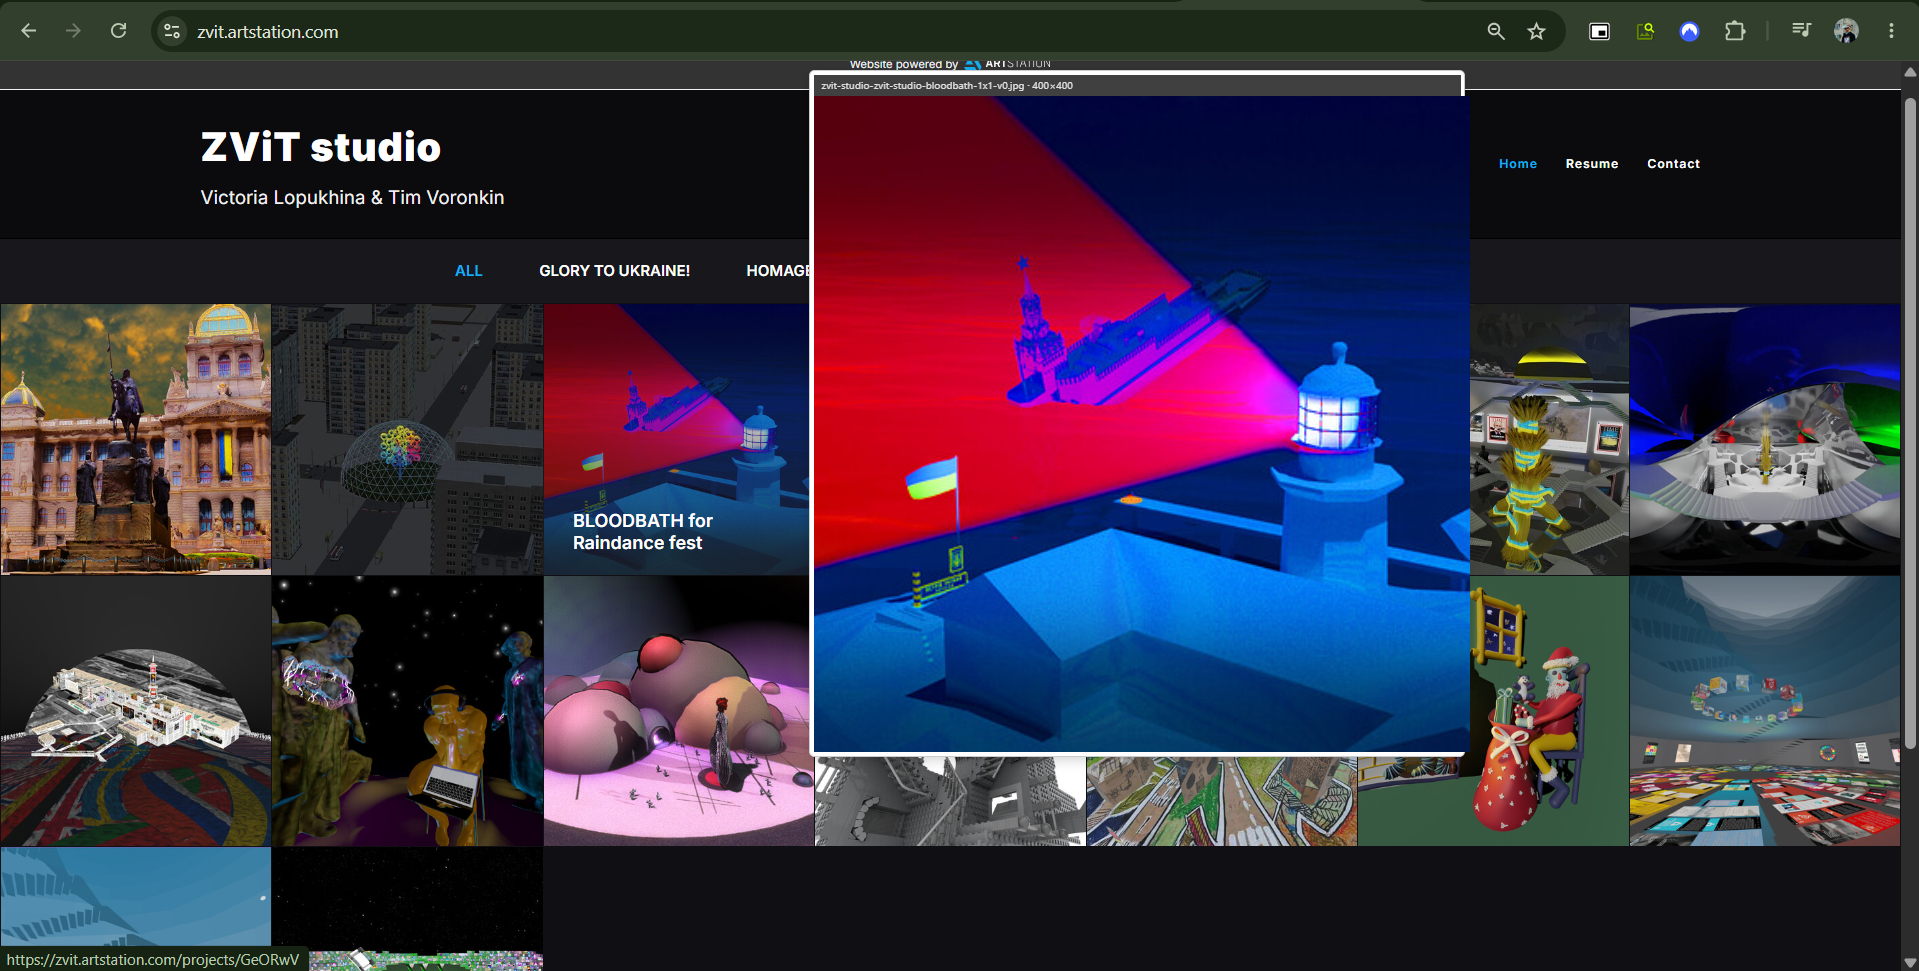
\includegraphics[width=0.9\textwidth]{img/scr_preview-img_on-zvit-studio.png}
    \caption{Náhled obrázku na portálu pro sdílení digitálního umění ArtStation}
    \label{fig:preview_img_artstation}
\end{figure}

\begin{figure}[htbp]
    \centering
    \includegraphics[width=0.9\textwidth]{img/scr_preview-svg_on-upce.png}
    \caption{Plynulý náhled vektorového obrázku (SVG) na portálu UPCE}
    \label{fig:preview_svg_upce}
\end{figure}

\subsection{Uživatelská příručka (Instalace a~konfigurace)}
\label{subsec:praxe_prirucka}

Vzhledem k~tomu, že rozšíření není v~době psaní práce publikováno ve veřejných obchodech s~doplňky (Chrome Web Store / Firefox Add-ons), probíhá jeho instalace prostřednictvím vývojářského režimu. 

\noindent\textbf{Postup instalace pro prohlížeče na bázi Chromium (Google Chrome, Edge, Brave):}
\begin{enumerate}
    \item Uživatel stáhne zdrojové kódy ve formátu ZIP a~rozbalí je do zvoleného adresáře.
    \item V~prohlížeči otevře stránku správy rozšíření zadáním adresy \texttt{chrome://extensions}.
    \item V~pravém horním rohu aktivuje přepínač \textbf{Režim pro vývojáře} (Developer mode).
    \item Klikne na tlačítko \textbf{Načíst rozbalené} (Load unpacked) a~vybere složku \texttt{src} z~rozbaleného archivu.
    \item Rozšíření je tímto nainstalováno a~jeho ikona se objeví na hlavní liště.
\end{enumerate}

Po úspěšné instalaci může uživatel kliknout na ikonu rozšíření a~otevřít vyskakovací okno (Popup) pro okamžitou správu stavu, nebo přejít do nastavení (Options) kliknutím pravým tlačítkem myši na ikonu a~volbou \textit{Možnosti}. Zde lze přidávat vlastní domény do allowlistu či blocklistu.

\subsection{Limity stávajícího řešení a~budoucí vývoj}
\label{subsec:praxe_limity}

Přestože navržené řešení úspěšně splňuje definované cíle, existují v~současné verzi určité technické a~funkční limity, které by mohly být předmětem dalšího vývoje:

\begin{itemize}
    \item \textbf{Podpora kancelářských formátů:} V~současnosti systém nativně renderuje primárně formáty běžných obrázků (JPEG, PNG, SVG, WebP) a~dokumenty PDF. Rozšíření o~podporu kancelářských dokumentů typu \texttt{.docx}, \texttt{.xlsx} nebo \texttt{.pptx} by výrazně zvýšilo užitnou hodnotu, avšak vyžadovalo by integraci dalších komplexních knihoven nebo využití externích cloudových API (např. Google Docs Viewer), což s~sebou nese rizika z~hlediska ochrany soukromí.
    \item \textbf{Výkon u~gigantických souborů:} Ačkoliv integrace \textit{PDF.js} probíhá přes nezávislé vlákno (Web Worker), u~extrémně objemných PDF souborů (stovky megabytů dat s~komplexní vektorovou grafikou) může docházet ke zpoždění při stahování a~úvodním renderování první strany. Zavedení inteligentního streamování a~využití HTTP hlaviček \texttt{Range} by tento proces optimalizovalo.
    \item \textbf{Přehrávání multimédií:} Konkurenční řešení často podporují náhledy animovaných GIFů nebo videí. Současná verze rozšíření se videím záměrně vyhýbá kvůli snížení paměťové náročnosti a~zamezení rušivému přehrávání zvuku (autoplay), avšak do budoucna lze implementovat volitelný modul pro ztlumené přehrávání oblíbených video formátů.
\end{itemize}

V~dalším vývoji je rovněž v~plánu publikovat rozšíření v~oficiálních obchodech doplňků, čímž by se zjednodušil proces instalace pro běžné uživatele a~zajistila by se automatická aktualizace softwaru.

%%%%%%%%%%%%%%%%%%%%%%%%%%%%%%%%%%%%%%%%%%%%%%%%%%%%%%%%%%%%
% ZÁVĚR
%%%%%%%%%%%%%%%%%%%%%%%%%%%%%%%%%%%%%%%%%%%%%%%%%%%%%%%%%%%%

\section*{Závěr}

Cílem této bakalářské práce bylo navrhnout a~implementovat moderní rozšíření pro webové prohlížeče, které zefektivní práci s~online obsahem tím, že uživatelům umožní okamžité zobrazení náhledů obrázků a~dokumentů PDF pouhým najetím kurzoru myši.

V~teoretické části byly popsány mechanismy asynchronního programování, zpracování událostí v~rámci DOM struktury a~limity současných technologických standardů. Tyto poznatky byly následně aplikovány v~praktické části při vývoji samotného softwarového modulu. Výsledkem je plně funkční, responzivní a~výkonnostně optimalizované rozšíření \textit{Interactive Previews}, které bezpečně integruje knihovnu PDF.js pro vykreslování vícestránkových dokumentů a~nabízí uživateli rozsáhlé možnosti personalizace prostřednictvím regulárních výrazů (filtrování domén).

Testování na produkčních webech potvrdilo, že navržené řešení eliminuje nutnost neustálého klikání a~stahování souborů za účelem rychlé inspekce jejich obsahu, čímž prokazatelně šetří čas a~zvyšuje plynulost prohlížení webu. Z~hlediska budoucího vývoje se nabízí možnost integrace podpory dalších komplexních kancelářských formátů, například DOCX, ODT, ODS či XLSX, a~implementace analytických nástrojů pro měření průměrné časové úspory koncových uživatelů.


%%%%%%%%%%%%%%%%%%%%%%%%%%%%%%%%%%%%%%%%%%%%%%%%%%%%%%%%%%%%
% POUŽITÁ LITERATURA
%%%%%%%%%%%%%%%%%%%%%%%%%%%%%%%%%%%%%%%%%%%%%%%%%%%%%%%%%%%%

%%%%%%%%%%%%%%%%%%%%%%%%%%%%%%%%%%%%%%%%%%%%%%%%%%%%%%%%%%%%
% BibLaTeX

\ifVSKPusesBibLaTeX					% při použití BibLaTeXu

\printbibliography

\else								% při nepoužití BibLaTeXu

%%%%%%%%%%%%%%%%%%%%%%%%%%%%%%%%%%%%%%%%%%%%%%%%%%%%%%%%%%%%
% pokud není použit biblatex:

% VZOR:
%\begin{thebibliography}{99}	% parametr určuje nejširší položku
%\sloppy\latexraggedright
%% nezlomitelné spojovníky lze zapisovat zkratkou "- nebo příkazem \babelhyphen{nobreak}
%
%\bibitem{bib:iso690pdf2011}
%	\textsc{Biernátová}, Olga a~Jan \textsc{Skůpa}.
%	\textit{Bibliografické odkazy a~citace dokumentů dle ČSN~ISO~690~(01~0197) platné od 1.\,dubna~2011}. Online.
%	Brno, 2.\,9.\,2011.
%	Dostupné z:~\url{http://www.citace.com/CSN-ISO-690.pdf} [cit.\,2016"-07"-29].
%
%\bibitem{bib:kocicka2004}
%	\textsc{Kočička}, Pavel a~Filip \textsc{Blažek}.
%	\textit{Praktická typografie}.
%	2.\,vyd.
%	Brno: Computer Press, 2004.
%	ISBN 80"-7226"-385"-4.
%	
%\bibitem{bib:lukes2017}
%	\textsc{Lukeš}, Lubomír.
%	\textit{Úroveň podpory typografie v~současných kancelářských editorech}.
%	Pardubice, 2017.
%	Diplomová práce. Univerzita Pardubice. Vedoucí práce Tomáš \textsc{Hudec}.
%
%\end{thebibliography}

\fi									% else: při použití BibLaTeXu


%%%%%%%%%%%%%%%%%%%%%%%%%%%%%%%%%%%%%%%%%%%%%%%%%%%%%%%%%%%%
% PŘÍLOHY
%%%%%%%%%%%%%%%%%%%%%%%%%%%%%%%%%%%%%%%%%%%%%%%%%%%%%%%%%%%%

% SEZNAM PŘÍLOH

\listofappendices

%%%%%%%%%%%%%%%%%%%%%%%%%%%%%%%%%%%%%%%%%%%%%%%%%%%%%%%%%%%%
%\normalparfillskip
%\noparindent[.5]					% odstavce bez zarážky, půl řádku vynechávat

% reset číslování pro přílohy, volitelný parametr je makro pro úpravu titulku např. pro verzálky [\MakeUppercase]
\backmatter%[\MakeUppercase]

%%%%%%%%%%%%%%%%%%%%%%%%%%%%%%%%%%%%%%%%%%%%%%%%%%%%%%%%%%%%
% PŘÍLOHA A
\appendix{Struktura souborů projektu}
\label{priloha:struktura}

Vývojový adresář projektu je logicky rozdělen do několika složek podle funkce jednotlivých komponent rozšíření. Níže je uvedena zjednodušená stromová struktura repozitáře s~popisem klíčových souborů a~adresářů:

\begin{lstlisting}[language={}, numbers=none, basicstyle=\ttfamily\small]
Interactive-Previews/
|-- assets/                # Statické soubory (ikony aplikace)
|-- Documentation/         # Zdrojové soubory textu bakalářské práce (LaTeX)
|-- src/                   # Zdrojové kódy samotného rozšíření
|   |-- background/        # Skripty běžící na pozadí (Service Worker)
|   |-- common/            # Sdílené konstanty a pomocné funkce
|   |-- content/           # Skripty a styly vkládané do stránek (DOM logika)
|   |-- options/           # Konfigurační rozhraní (Options)
|   |-- pdfjs/             # Knihovna PDF.js pro vykreslování PDF
|   `-- popup/             # Vyskakovací okno rozšíření (Popup)
|-- manifest.json          # Hlavní konfigurační soubor rozšíření
`-- README.md              # Základní informace o projektu
\end{lstlisting}

%%%%%%%%%%%%%%%%%%%%%%%%%%%%%%%%%%%%%%%%%%%%%%%%%%%%%%%%%%%%
% PŘÍLOHA B
\appendix{Konfigurační soubor manifest.json}
\label{priloha:manifest}

Klíčový soubor \texttt{manifest.json} (dle specifikace Manifest V3), který definuje základní metadata rozšíření, potřebná oprávnění (např.~\texttt{activeTab}) a~cesty k~jednotlivým komponentám (Service Worker, Content Scripts atd.).

\begin{lstlisting}[language=JavaScript, numbers=none, basicstyle=\ttfamily\footnotesize]
{
  "manifest_version": 3,
  "name": "Interactive Previews",
  "version": "1.0",
  "description": "Shows interactive previews of images and documents on hover.",
  "permissions": [
    "storage",
    "activeTab"
  ],
  "host_permissions": [
    "<all_urls>"
  ],
  "background": {
    "service_worker": "src/background/background.js"
  },
  "action": {
    "default_popup": "src/popup/popup.html"
  },
  "options_ui": {
    "page": "src/options/options.html",
    "open_in_tab": true
  },
  "content_scripts": [
    {
      "matches": ["<all_urls>"],
      "js": [
        "src/pdfjs/pdf.min.js",
        "src/content/utils.js",
        "src/content/info-bar.js",
        "src/content/preview-image.js",
        "src/content/preview-pdf.js",
        "src/content/content.js"
      ],
      "css": ["src/content/content.css"]
    }
  ],
  "web_accessible_resources": [
    {
      "resources": ["src/pdfjs/pdf.worker.min.js"],
      "matches": ["<all_urls>"]
    }
  ]
}
\end{lstlisting}

%%%%%%%%%%%%%%%%%%%%%%%%%%%%%%%%%%%%%%%%%%%%%%%%%%%%%%%%%%%%%
%% PŘÍLOHA C
%\appendix{Soubor metadat XMP v~PDF}
%\label{priloha:xmp}
%
%Obsah souboru s~metadaty ve formátu XMP. Vyžadováno pro archivaci ve formátu PDF/A.
%
%\VerbatimInput[breaklines=true, fontsize=\small]{\jobname.xmpdata}

%%%%%%%%%%%%%%%%%%%%%%%%%%%%%%%%%%%%%%%%%%%%%%%%%%%%%%%%%%%%
% KONEC DOKUMENTU
%%%%%%%%%%%%%%%%%%%%%%%%%%%%%%%%%%%%%%%%%%%%%%%%%%%%%%%%%%%%

\end{document}

% vim:sw=8:ts=8
% EOF